
Die Detaillierung des Entwurfes basiert größtenteils auf den Spezifikationen und Maßen verfügbarer Kaufteile und Abschätzungen für gewählte Abmessungen anhand von Ausführungen oder Beispielen in den herangezogenen Veröffentlichungen. Dabei sind vor allem~\cite{Design_of_shielded_enclosures, EMV-gerechtes_Geraetedesign, EM_Schirmung, Simplified_shielding, Handbook_Shielding_Materials_and_Performance} zu nennen, die als Referenz dienten. Die folgenden Ausführungen schildern das Ergebnis des Konstruktionsprozesses in einer möglichst systematischen Reihenfolge.

\subsection{Verwendete Messtechnik}

Die Hauptkomponente der verwendeten Messtechnik stellt, wie bereits erwähnt, ein \ac{VNA} dar. Der für diese Arbeit zur Verfügung stehende \ac{VNA} der Firma Anritsu ist ein Zweikanal-Netzwerkanalysator mit einem Arbeitsbereich zwischen \SI{1}{\mega\hertz} und \SI{20}{\giga\hertz}. Ein Auszug mit den für dieses Modell relevanten Daten und Diagrammen nach~\cite{VNA-Datenblatt} ist im \Anhang\ref{A:Datenblatt_VNA} zu finden. 
\par
\vspace{\linespace}
Da der \ac{VNA} mithilfe der zwei verfügbaren Ports sowohl die Sendeantenne speist als auch das Messsignal an der Empfangsanatenne aufnimmt, kann die Ermittlung der Schirmdämpfung direkt durch die zugehörige Software erfolgen. Außerdem wären Zeitbereichsmessungen (Time Domain Measurements) möglich, wodurch eine Unterscheidung zwischen dem direkten und indirekten Koppelpfad möglich wäre~\cite{Techniques_Shielding_Effectiveness_Far_Field_Simulation}. %Im \Kapitel\ref{cha:4} wird darauf näher eingegangen.
\par
\vspace{\linespace}
% Die Kalibration der Messtechnik erfolgt mithilfe des zugehörigen Kalibrationskits, wodurch bei korrekter Durchführung die im Auszug des Datenblattes (vgl. \Anhang\ref{A:Datenblatt_VNA}) dargestellten Unsicherheiten eingehalten werden sollten. Auf die durchgeführte Kalibration des \ac{VNA} wird im \Abschnitt\ref{cha:4_Kalibration_Messtechnik} näher eingegangen.
% \par
% \vspace{\linespace}
Die Verbindung des \ac{VNA} erfolgt mittels der zugehörigen Signalkabel, die eine Wellenimpedanz von \SI{50}{\ohm} aufweisen~\cite{Testkabel_VNA-Datenblatt}. Die Anschlüsse sind \ac{SMA} kompatible Steckverbinder mit \SI{2,92}{\milli\meter}-Stecker.
\par
\vspace{\linespace}
%Antennen/Waveguides
    %Größe
    %Platziert mit vorhandenen Stativen
Die zur Verfügung stehenden Antennen sind Breitband-Hornstrahler mit einer linearen Polarisation und den in der \Tabelle\ref{tab:3_Spezifikationen_Antennen} zusammengefassten wichtigsten Spezifikationen nach~\cite{Antennen-Datenblatt}. Weitere Kenndaten sind im \Anhang\ref{A:Datenblatt_Antennen} zu finden. Die Antennen bieten ebenfalls einen SMA-Anschluss für die Signalkabel, welche nach~\cite{DIN_EN_61000-5-7} so ausgeführt sind, dass ihre Kopplungsdämpfung mit garantierten \SI{95}{\Dezibel}~\cite{Pasternack_Koaxkabel_PE-P142LL} deutlich über der zu messenden Schirmdämpfung liegt, wie an den Messwerten der Referenzmessungen in~\cite{FSS_Toedter_Diplomarbeit} erkennbar ist.  

\begin{table}[ht]
    \centering
    \caption[Technische Spezifikationen der verwendeten Hornstrahler]{Technische Spezifikationen der verwendeten Hornstrahler nach~\cite{Antennen-Datenblatt}}
    \label{tab:3_Spezifikationen_Antennen}
    \vspace{\tablespace}
    \begin{tabular}{p{6cm} p{4cm}}
    \toprule
        \textbf{Spezifikation} & \textbf{Wert} \\
    \midrule
        Frequenzbereich & $0,8 - 18\;\si{\giga\hertz}$ \\
        Halbwerts-Strahlbreite  & $111-13 \;\si{\degree}$ (E-Feld) \\
                                & $78-10\;\si{\degree}$ (H-Feld) \\
        Kreuzpolarisation-Isolation & \SI{25}{\Dezibel} (typ.) \\
        Stehwellenverhältnis (VSWR) & $1,5 : 1$ (typ.) \\
        Abmessungen             & $244\times160,5\times228\;\si{\milli\meter}$ \\
    \bottomrule
    \end{tabular}
\end{table}

Mit den vorhandenen Aluminium-Stativen können die Antennen frei auf einer Höhe zwischen \SI{53}{\centi\meter} und \SI{158}{\centi\meter} platziert werden, was eine Positionierung in der Messkabine entsprechend der Anforderungen erlaubt.




\subsection{Konstruktion}\label{cha:3_sub_Konstruktion}

Die Modulwände werden hauptsächlich aus den Sandwichpaneelen gebildet, wodurch deren Auswahl von zentraler Bedeutung für die restliche Konstruktion ist. Aufgrund von Produktverfügbarkeiten mussten Verbundplatten aus Sperrholz mit metallischen Deckblechen, wie sie im Rahmen professioneller Absorberkammern zum Einsatz kommen, schon zu Beginn der Konzeptphase verworfen werden. Als Alternative wurden Wabenkernplatten gewählt, welche ebenfalls durchgehende Deckbleche besitzen, aufgrund ihrer inneren Struktur ein deutlich günstigeres Verhältnis aus Biegesteifigkeit und Gewicht besitzen und auf ganz ähnliche Weise verarbeitet werden können~\cite{Alucore-Datenblatt}. Im Messbereich zwischen 1 -- \SI{18}{\giga\hertz} ist nach \Abschnitt\ref{cha:2_sub_Schirmung_ebener_Wellenfelder} die Absorptions- und Reflektionsdämpfung für die kombinierten \SI{2}{\milli\meter} Blechstärke bereits so hoch, dass für die real erreichte Schirmung des Versuchsstandes gegenüber Störquellen von außen nur noch Öffnungen wie Türen oder Verbindungsstellen entscheidend sind.  
\par
\vspace{\linespace}
Für den vorgesehenen Einsatzzweck musste die Polyesterlackschicht an allen Wirkflächen, das heißt allen Verbindungsflächen der Modulwände untereinander und allen weiteren Anschlussflächen, mechanisch entfernt werden. Um trotz der sich stets an Luftatmosphäre bildenden Oxidschichten einen leitfähigen Kontakt an allen Wirkflächen herzustellen, wurden Funktionselemente nach Möglichkeit miteinander verschraubt. Dabei kann im Fall von Aluminium bereits bei Vorspannkräften in einer Größenordnung von \SI{1000}{\newton} davon ausgegangen werden, dass die harten Oxidschichten aufreißen und Metall-Metall-Kontakt entsteht~\cite{Projektarbeit}. Aus diesem Grund wurde unter anderem ebenfalls von der Verwendung von Nieten abgesehen, wobei ein weiterer Grund die theoretische Möglichkeit eines Umbaus oder einer Erweiterung bei Verwendung lösbarer Verbindungen war. Weiterhin nutzen Schraubenverbindungen im Fall der Modulwände die Wabenstruktur Sandwichpaneele besser aus, was zu einer deutlich erhöhten Stabilität führt, als dies bei einer Vernietung der Fall wäre. An den Türen gewährleisten die gewählten HF-Dichtungen aufgrund der Relativbewegung bei jedem Schließvorgang eine mechanische Entfernung der Oxidschichten.
\par
\vspace{\linespace}
Die Grundlage für die Auslegung der L-Profile entsprechend des gewählten Wirkkonzeptes für die Modulwände bildete der aus der Schraubenberechnung bekannte Rötscher-Kegel. Die Schenkellänge der Profile, welche die Wabenkernplatten an den Eckstößen miteinander verbinden, wurden nach den verfügbaren Profilmaßen so gewählt, dass sich der Verspannungskegel innerhalb der verschraubten Teile vollständig ausbilden kann und somit die Vorspannkraft der Schrauben möglichst großflächig in die Wabenkernplatte eingeleitet wird. Die \Abb\ref{fig:3_Verspannungskegel_L-Profile} zeigt dies in einer schematischen Darstellung zusammen mit den gewählten Profilmaßen und dem sich ergebenden Ersatzquerschnitt des Schraubverbandes. 

\begin{figure}[ht]
    \centering
    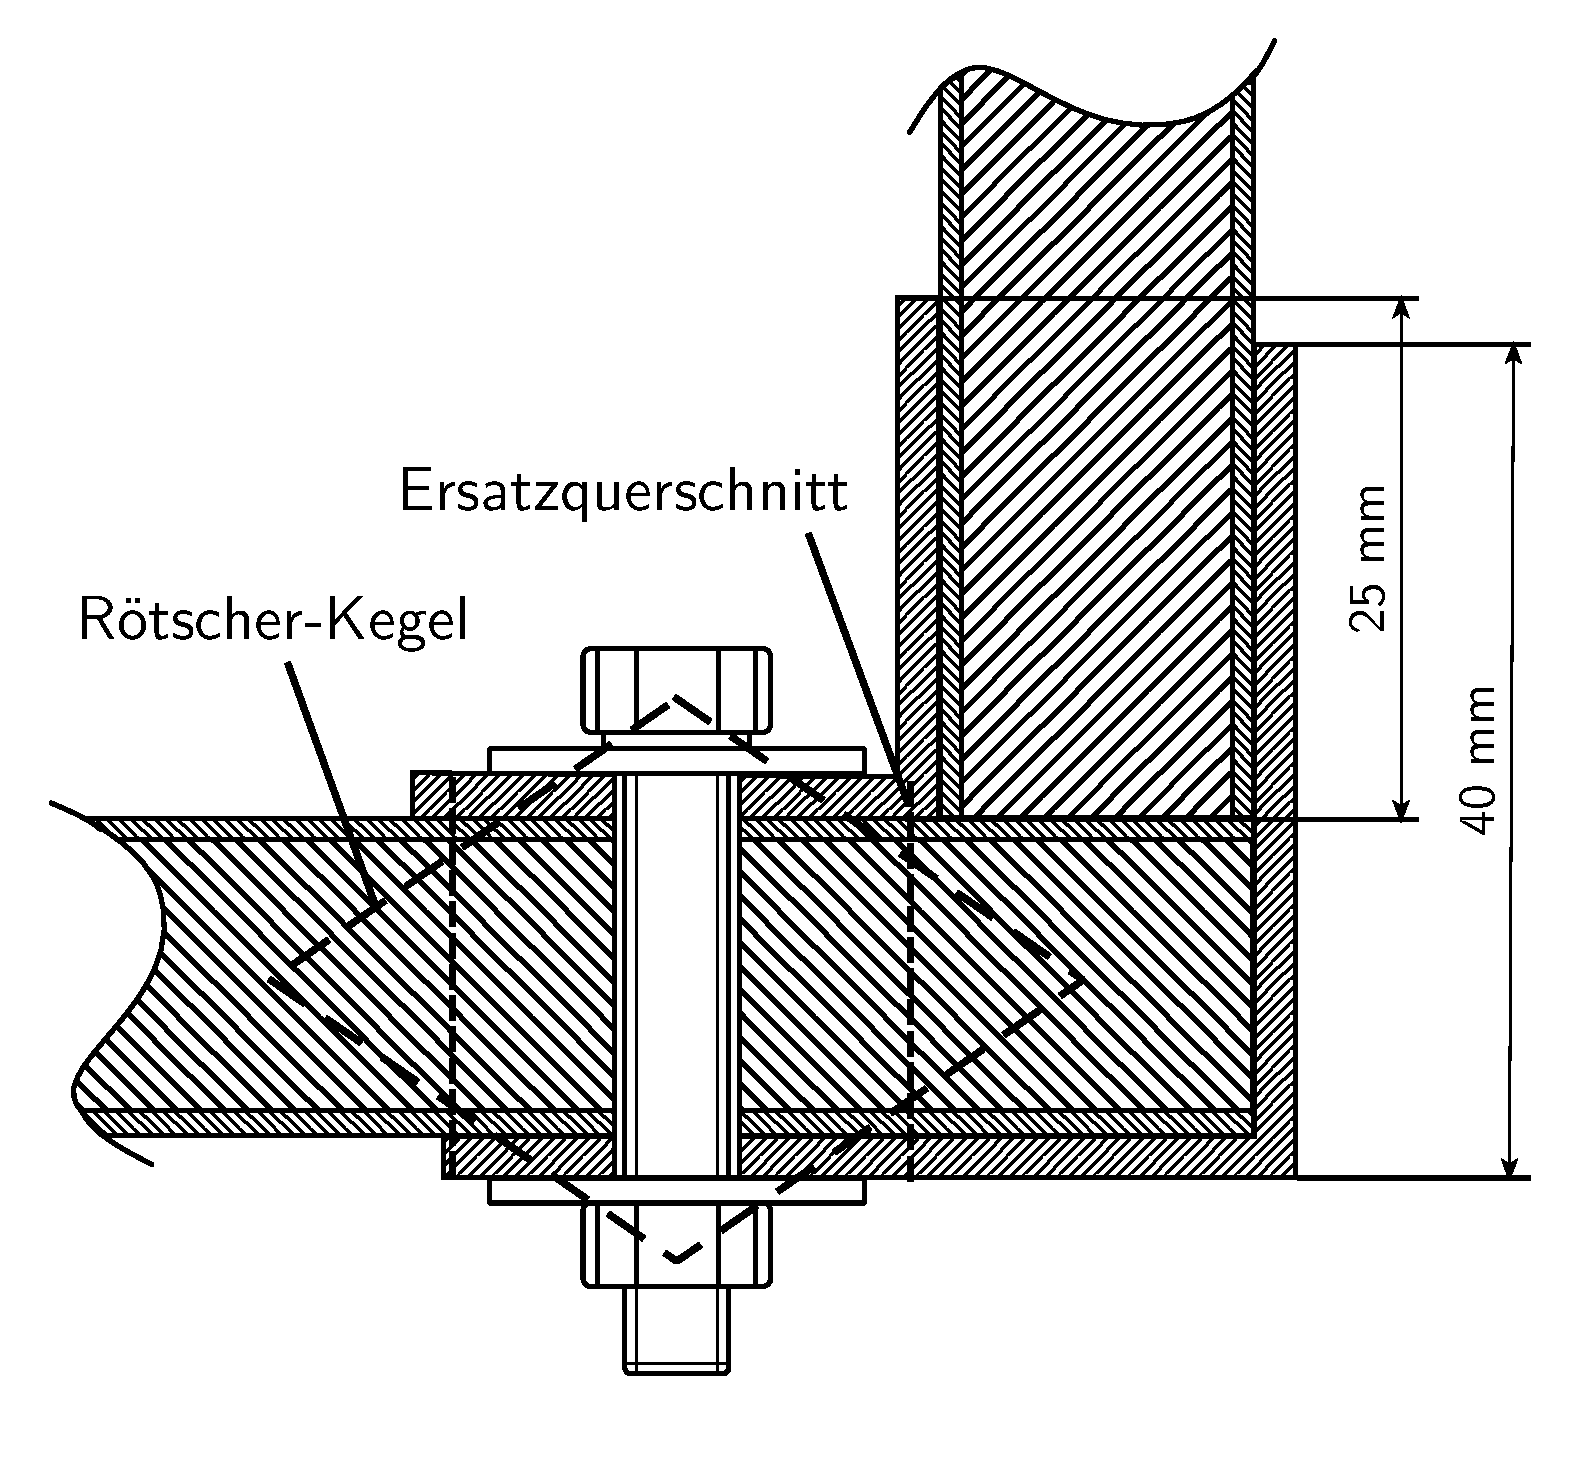
\includegraphics[page=1, trim=1cm 1.5cm 1cm 1cm, clip, width = .45\textwidth]{Abbildungen/Kapitel3/Schematik_Verspannungskegel.pdf}
    \caption{Schematische Darstellung des Verspannungsbereiches der verschraubten Modulwände}
    \label{fig:3_Verspannungskegel_L-Profile}
\end{figure}


Die Wahl des Schraubenabstandes wurde auf Grundlage eines Zusammenhanges nach~\cite{Design_of_shielded_enclosures} getroffen, welcher die erreichbare Schirmdämpfung als Funktion des Schraubenabstandes verschraubter Blechteile darstellt. Wie aus der Grafik in \Abb\ref{fig:3_Schirmwirkung_Schraubenabstand} hervorgeht, kann bei einem Schraubenabstand von \SI{10}{\centi\meter} von etwa \SI{70}{\Dezibel} theoretisch erreichbarer Schirmdämpfung je Funktionsfläche ausgegangen werden. Dieser Abstand wurde auch in Hinblick auf den Fertigungsaufwand der Bohrungen und Verschraubungen gewählt. Aufgrund der Sandwichbauweise der Modulwände befinden sich des Weiteren stets zwei versetzt verschraubte Wirkflächen im Koppelpfad, wodurch der Durchgriff weiter verringert wird. Die Anfertigung der Bohrungen erfolgte händisch und während des Zusammenbauprozesses, um eine möglichst exakte Ausrichtung der Bohrlöcher in den einzelnen verspannten Teilen relativ zueinander zu erreichen. Die Berechnung des Anzugsmomentes der Schrauben unter Beachtung der Druckfestigkeit der Wabenkernplatten stellte sicher, dass keine plastische Verformung des Wabenkerns erfolgte und die Wirkfläche somit eben blieb. Von der Verwendung selbstschneidender Schrauben wurde aufgrund der Gefahr verformter Gewinde und damit unsauberer Verbindungsstellen abgesehen.  
\par
\vspace{\linespace}\vspace{\linespace}

\begin{figure}[ht]
    \centering
    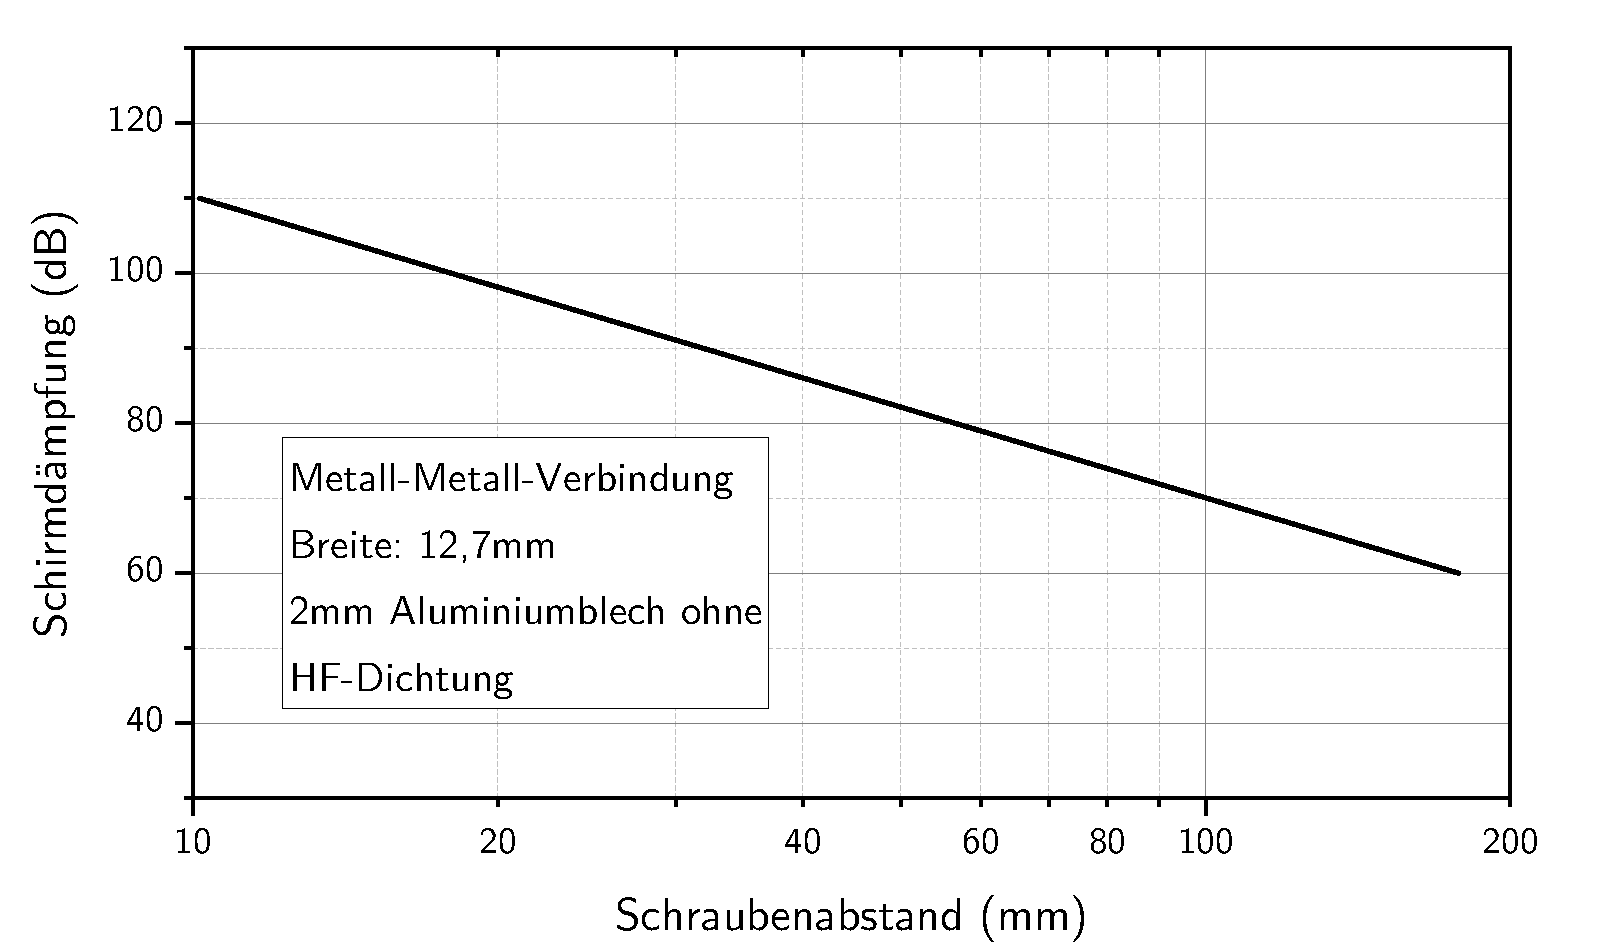
\includegraphics[page = 1, trim = 0cm 0cm 0cm 0cm, clip, width=.99\textwidth]{Abbildungen/Kapitel3/Schraubenabstand_Schirmwirkung.pdf}
    \caption[Schirmdämpfung verschraubter Blechteile in Abhängigkeit des Schraubenabstandes]{Schirmdämpfung verschraubter Blechteile in Abhängigkeit des Schraubenabstandes nach~\cite{Design_of_shielded_enclosures}}
    \label{fig:3_Schirmwirkung_Schraubenabstand}
\end{figure}


Um eine möglichst hohe Schirmdämpfung zu erreichen, wurde die Anordnung der Profile mit entsprechenden Aussparungen so gewählt, dass sich an keiner Stelle zwei Anschlussstellen im Koppelpfad von äußeren Störquellen nach innen direkt gegenüberstehen. Dies führt zu einer Labyrinthwirkung an Stellen von Profilübergängen und verringert somit ebenfalls den Felddurchgriff. Zusätzlich wurden auf der Innenseite alle Verbindungsstellen mit leitfähigem Aluminiumband versehen. Mit dem gewählten Konzept und Schraubenabstand wäre eine höhere Schirmwirkung an den Verbindungsstellen der Profile untereinander nur durch dichtes Verschweißen oder Verlöten zu erreichen~\cite{Design_of_shielded_enclosures, EM_Schirmung}, was jedoch schon zu Beginn der Konzeptphase aufgrund der Fertigbarkeit und unlösbaren Verbindung der Modulelemente als Fertigungsverfahren verworfen wurde. 
\par
\vspace{\linespace}


%Wabenkernplatten als Grundlage 
    %Verfügbarkeit
    %Vorteile gegenüber Vollmaterial (ggf. mit Grafik bzw. Wert
    %Datenblatt ggf. einfügen
    %Besonderheiten (Entfernen der Lackschicht z.B.)
    
%Aluprofile mit Rechnung bzw. der gewählten Dicke und Maßen

%Schraubenberechnung ggf.

%(Aufbau-(Reigenfolge))


Die Auswahl geeigneter Absorberelemente wurde unter Einbeziehung der erreichbaren Reflektionsdämpfung, der Höhe einzelner Elemente und ökonomischen Gesichtspunkten getroffen. Die Reflektionsdämpfung gibt hierbei das Verhältnis einer eintreffenden Welle zum reflektierten Anteil an. Eine möglichst hohe und gleichbleibende Reflektionsdämpfung über alle Einsatzfrequenzen ist dementsprechend wünschenswert. Im \Abschnitt\ref{cha:3_Entwurf} wurde die Auswahl bereits auf reine Pyramidenabsorber eingeschränkt. Zur Vermeidung von reflektivem Verhalten bei hohen Frequenzen sollten keine Absorberelemente mit abgeschnittener Spitze verwendet werden. 
\par
\vspace{\linespace}
Die gewählten Absorber besitzen die in \Tabelle\ref{tab:3_Reflektionsdaempfung_Absorberelemente} angegebene garantierte Reflektionsdämpfung im Messbereich dieser Arbeit. Mit einer Höhe von \SI{10}{\centi\meter}  verbleibt auch nach dem Einbau noch ein großer Messbereich in der Testkammer. Des Weiteren ist vor allem im höheren Frequenzbereich eine höhere Reflektionsdämpfung zu erwarten, als bei der \SI{20}{\centi\meter} hohen Variante der gleichen Produktfamilie. Auf die Verwendung noch höherer Elemente wurde aufgrund der steigenden Einschränkung des Messraumes und aus ökonomischer Sicht verzichtet.  
\par
\vspace{\linespace}

\begin{table}[ht]
    \centering
    \renewcommand{\arraystretch}{1.2}
    \caption[Gemessene und garantierte Reflektionsdämpfung der verwendeten EPP12 Pyramidenabsorber im Bereich zwischen \SI{1}{\giga\hertz} bis \SI{18}{\giga\hertz}]{Gemessene und garantierte Reflektionsdämpfung der verwendeten EPP12 Pyramidenabsorber im Bereich zwischen \SI{1}{\giga\hertz} bis \SI{18}{\giga\hertz} nach~\cite{Eco_Messtechnik_Absorber}}
    \label{tab:3_Reflektionsdaempfung_Absorberelemente}    
    \vspace{\tablespace}
    \begin{tabular}{p{2cm} C{1.6cm} C{1.6cm} C{1.6cm} C{1.6cm} C{1.6cm}}
        \toprule
            &   \multicolumn{5}{l}{\textbf{Reflektionsdämpfung [\SI{}{\Dezibel}]}} \\
        \midrule
            &   \SI{1}{\giga\hertz} & \SI{3}{\giga\hertz} & \SI{5}{\giga\hertz} & \SI{10}{\giga\hertz} & \SI{18}{\giga\hertz} \\
        \textbf{Gemessen}   &   15  &   32  &   42  &   50  &   55 \\    
        \textbf{Garantiert} &   12  &   30  &   40  &   45  &   50 \\
        \bottomrule
    \end{tabular}

\end{table}

Auf dem Messprotokoll~\cite{Eco_Messtechnik_Absorber} sind außerdem keine ausgezeichneten Peaks oder Einbrüche des Dämpfungsverhaltens zu erkennen. In Bezug auf Kosten und Abmessungen bieten vergleichbare alternative Absorber ab etwa \SI{5}{\giga\hertz} nur eine um \SI{5}{\Dezibel} reduzierte Reflektionsdämpfung, was bei Betrachtung des Verhältnisses der Feldgrößen etwa einem Faktor 2 entspricht (vgl. \Tabelle\ref{tab:2_Relative_Pegel})~\cite{Holland_Shielding_Absorber}. Mit Ferritkacheln und zusätzlich darauf abgestimmten Hybridabsorbern kann zwar bereits im Frequenzbereich zwischen \SI{1}{\giga\hertz} bis \SI{3}{\giga\hertz} eine Reflektionsdämpfung von \SI{25}{\Dezibel} erreicht werden, jedoch ist mit dieser Kombination aufgrund der Impedanzabstimmung der PU-Absorber auf die Ferritkacheln bei höheren Frequenzen nur mit etwas mehr als \SI{30}{\Dezibel} zu rechnen, ab \SI{10}{\giga\hertz} sogar nur mit weniger als \SI{30}{\Dezibel}~\cite{Holland_Shielding_Absorber} mit teils stark ausgeprägten Peaks in bestimmten Frequenzbändern. Aus diesen Gründen wurden die Absorber des Typs EPP12 der Firma \Firma{ECO-Messtechnik GmbH und Co. KG} verwendet. 
\par
\vspace{\linespace}
Für die Verkleidung von schmalen Bereichen und als Führung für die Antennenkabel, um eine stets gleichbleibende Lage über alle Messungen zu gewährleisten, kamen zusätzlich Flachabsorber des Typs EPF15, ebenfalls von \Firma{ECO-Messtechnik GmbH und Co. KG}~\cite{Eco_Messtechnik_Absorber}, zum Einsatz. Die Auskleidung der Ecken erfolgte mit versetzt angeordneten, umgedrehten Pyramidenstreifen. Dadurch konnte die nicht von Absorbern bedeckte Fläche auf ein Minimum reduziert und für die orthogonal angeordneten Elemente eine plane Anschlussfläche gewährleistet werden (vgl. \Abb\ref{fig:3_Absorberplatzierung}).
\par
\vspace{\linespace}

\begin{figure}[ht]
    \centering
    \includegraphics[draft = false, height=.2\textheight]{Abbildungen/Kapitel3/DSC_4536.jpg}
    \hspace{1cm}
    \includegraphics[draft = false, height=.2\textheight]{Abbildungen/Kapitel3/DSC_4523.jpg}
    \caption[Platzierung der verwendeten Absorber in Eckbereichen und an Durchführungen]{Platzierung der verwendeten Absorberelemente in Eckbereichen und an den Durchführungen}
    \label{fig:3_Absorberplatzierung}
\end{figure}


Die Befestigung der Absorberelemente erfolgte mittels Klettbändern, um eine nachträgliche Justierung oder einen Austausch leicht zu ermöglichen. Zusätzlich wurden Pyramidenabsorber im indirekten Koppelpfad der Antennen auf dem Boden platziert, um ungewollte Interferenz des direkten und indirekten Strahls zu verringern. Nach~\cite{Vergleich_Absorberhalle_Groundplane} erschien eine vollständige Auskleidung des Bodens auch in Hinblick auf Fertigung und Begehbarkeit in Ausnahmefällen nicht sinnvoll. Im dort durchgeführten Vergleich zeigt sich oberhalb von \SI{90}{\mega\hertz} ein qualitativ gleicher Verlauf der gemessenen Schirmdämpfung mit einem betragsmäßigen Unterschied von etwa \SI{5}{\Dezibel}. Durch Platzierung von wenigen Absorbern auf dem Boden zwischen den Antennen kann dies noch weiter reduziert werden. Der Unterschied zu einer Vollabsorberhalle ist dann kaum vorhanden. Darauf deuten auch die Ergebnisse in~\cite{Optimierung_Feldhomogenitaet} hin.
\par
\vspace{\linespace}




%Absorberelementauswahl 
    %Datenblatt
    %Anzahl Abschätzung
    %Flachabsorber für Ecken
    %Befestigung
    

Die am Reflektor zwischen den Antennen, welcher aus dem gleichen Material wie die Schirmwände besteht, befestigte Probenhalterung besteht aus zwei Z-Profile, in welche der nachfolgend beschriebene Probehalter eingeführt werden kann. Dies ermöglicht einen leichten Austausch und eine Messung in zwei Polarisationsrichtungen ohne die Proben zwischendurch neu verschrauben zu müssen. Weiterhin wird durch die verwendete Halterung die gleiche feste Anlage am Reflektor unabhängig der Stärke der Proben gewährleistet. Dies ist in Hinblick auf die Verwendbarkeit der Messkammer für Folien und Schäume von Bedeutung, da beide Arten von Proben sehr unterschiedliche Dicken aufweisen. Dies ist auch für die Gestaltung des Probenhalters ausschlaggebend.
\par
\vspace{\linespace}
Zur sicheren Positionierung der Proben in der Halterung wurde eine Verschraubung gewählt. Zwischen den verschraubten Hälften des Probenhalters sollten ebenfalls HF-Dichtungen angebracht werden. Um trotz unterschiedlicher Probenkörperstärke ein sicheres Anliegen der Kontaktfederstreifen zu gewährleisten, wurden die beiden Teile des Probenhalters als Blechwannen ausgeführt. Damit ist eine gewisse Relativverschiebung zwischen den Hälften je nach verwendeter Probe möglich, ohne die Anpresskraft auf die HF-Dichtungen zu verringern. Mit der verwendeten Probenhalterung können somit ohne Einschränkung Proben zwischen $0-14\,\si{\milli\meter}$ und $21-35\,\si{\milli\meter}$ und einer Ausdehnung zwischen \SI{110}{\milli\meter}$\; \times \;$\SI{110}{\milli\meter} und \SI{130}{\milli\meter}$\; \times \;$\SI{130}{\milli\meter} vermessen werden, was den Anforderungen entsprechend der Anforderungsliste entspricht (vgl. \Abb\ref{fig:3_Probenhalterung_und_Reflektor}). 
\par
\vspace{\linespace}
Die Öffnung des Reflektors wurde unter Beachtung der Fresnel-Ellipse der Übertragung zwischen den Antennen~\cite{Taschenbuch_HF-Technik} etwas größer gewählt als die Öffnung des Probenhalters, um den direkten Koppelpfad nicht zusätzlich zu beinträchtigen (vgl. \Abb\ref{subfig:3_Probenhalter_Konfig1}). Die Fresnelzone der Funkübertragung ist ein Ellipsoid, in welchem Hindernisse die Ausbreitung elektromagnetischer Wellen aufgrund der Wellencharakteristik stören können, auch wenn direkte Sichtverbindung besteht. Im Bereich der ersten Fresnelzone wird der Großteil der Strahlungsenergie übertragen. Verdeckungen innerhalb dieser führen aufgrund von destruktiven Interferenzen zur Dämpfung des Signals an der Empfangsantenne, da direkte und indirekte reflektierte Strahlen eine Phasendifferenz von bis zu einer halben Wellenlänge aufweisen~\cite{Advanced_Elecronic_Communication_Systems}. Aufgrund der Probengröße ist eine Interaktion des Probenhalters mit der Fresnelellipse erster Ordnung bei niedrigen Frequenzen nicht zu vermeiden, da diese schon bei geringsten Abständen zu Empfangsantenne einen Radius deutlich größer als \SI{10}{\centi\meter} aufweist. Der Radius der n-ten Fresnelzone lässt sich dabei mithilfe der Antennenabstände $d_1$ und $d_2$ von der Probe abschätzen~\cite{Taschenbuch_HF-Technik}:

\begin{equation}
    r^F_n = \sqrt{\frac{n\cdot \lambda\cdot d_1 \cdot d_2}{d_1 + d_2}}
    \label{Fresnelzone}
\end{equation}

\par
\vspace{\linespace}
Der Reflektor wurde mittels eines Gestells aus Holz in der Kammer platziert, um die Beeinträchtigung der Feldhomogenität zu minimieren. Durch möglichst genaue Messungen wurden die Anforderungen hinsichtlich der Positionierung von Antennen und Reflektor sichergestellt.
\par
\vspace{\linespace}

\begin{figure}[ht]
    \centering
    \begin{subfigure}[b]{0.9\textwidth}
        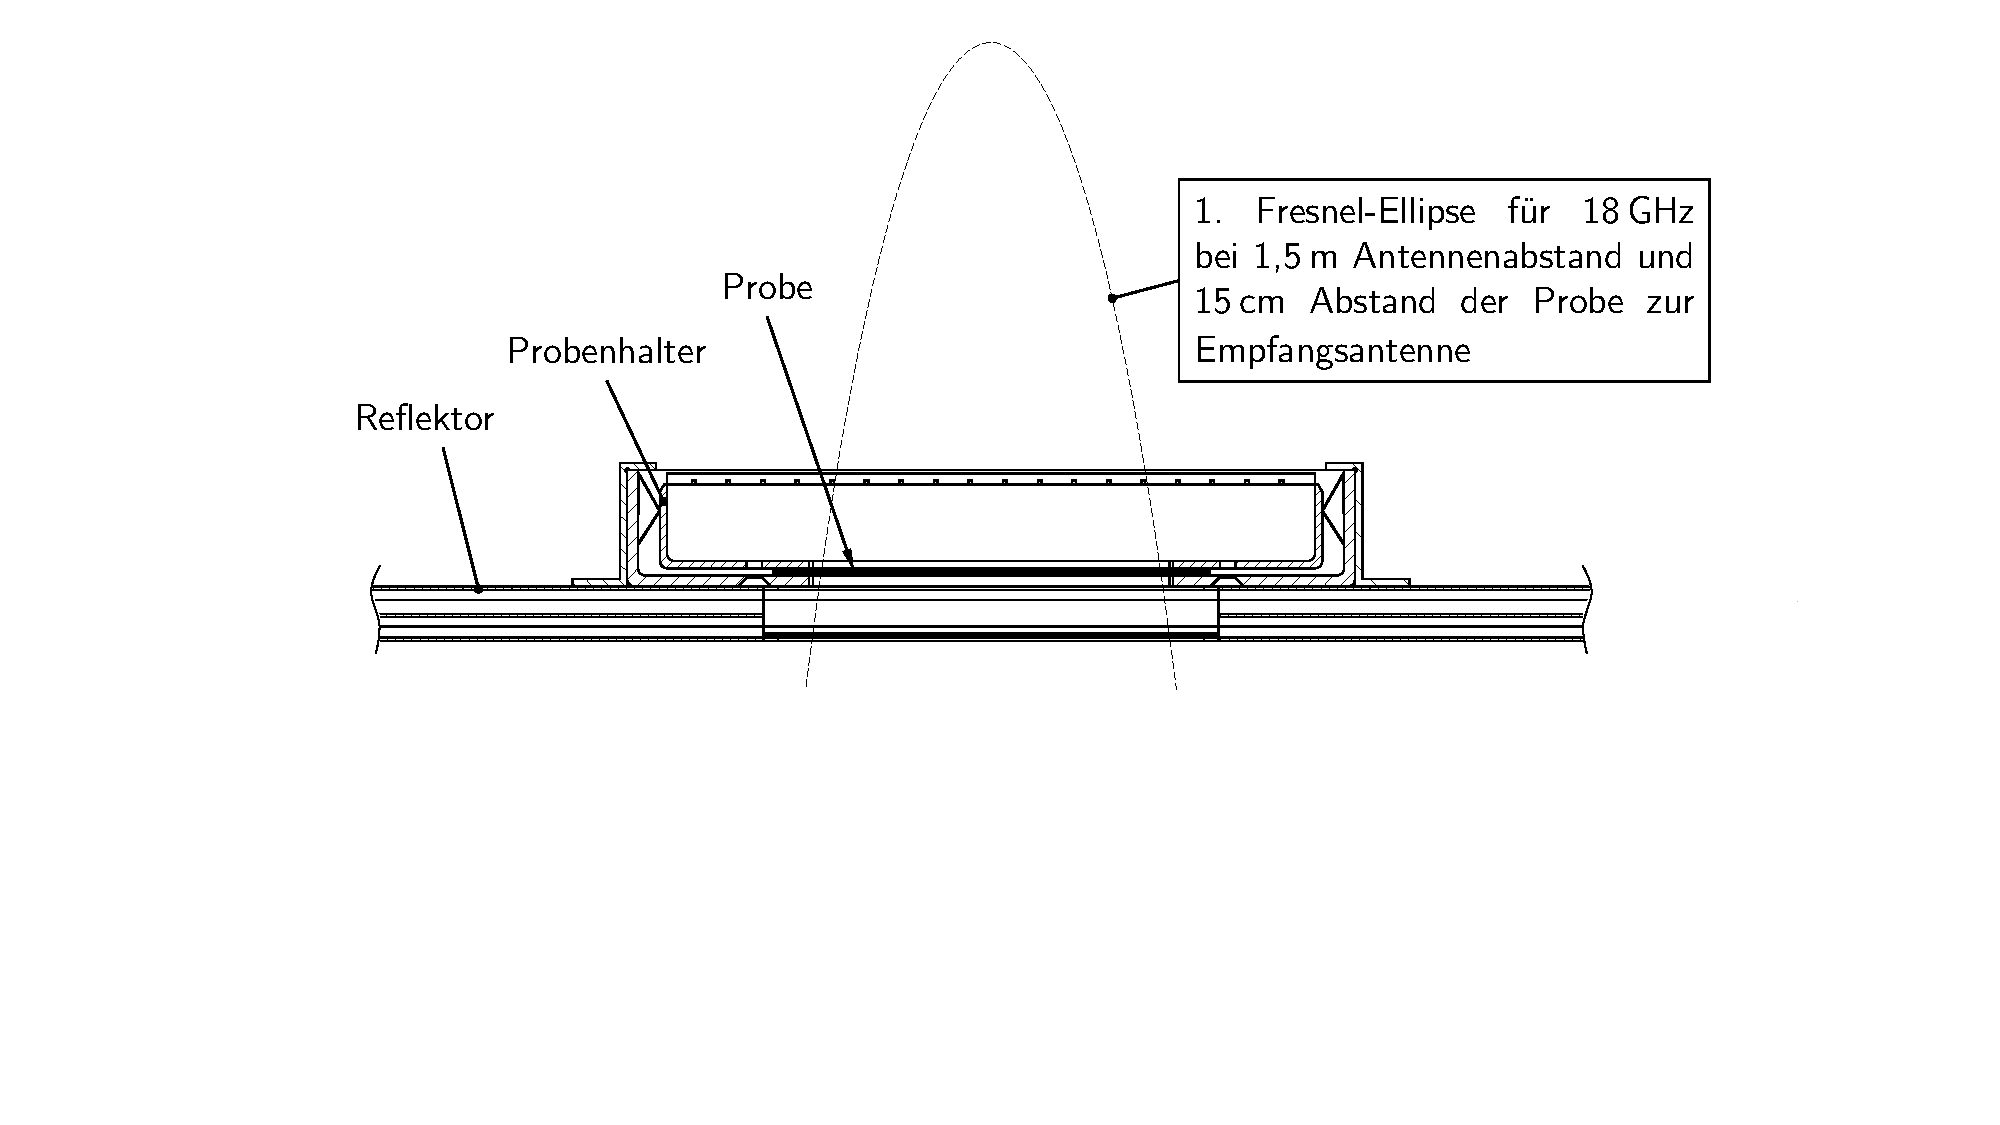
\includegraphics[page = 1, width=\textwidth, trim = 4.3cm 7cm 4.8cm 0cm, clip]{Abbildungen/Kapitel3/Probenhalter.pdf}
        \caption{Konfiguration 1 für Proben bis \SI{14}{\milli\meter} mit erster Fresnel-Ellipse}\label{subfig:3_Probenhalter_Konfig1}
    \end{subfigure}
    \hspace{2cm}
    \begin{subfigure}[b]{0.85\textwidth}
        \includegraphics[page = 2, width=\textwidth, trim = 5cm 7cm 5.5cm 7cm, clip]{Abbildungen/Kapitel3/Probenhalter.pdf}
        \caption{Konfiguration 2 für Proben bis \SI{35}{\milli\meter}}\label{subfig:3_Probenhalter_Konfig2}
    \end{subfigure}
    \caption{Schematische Darstellung der Probenhalterung in den möglichen Konfigurationen}
    \label{fig:3_Probenhalterung_und_Reflektor}
\end{figure}
    
%Probenreflektor mit Probenhalterung (CAD ggf.) und Beschreibung der Probenhalterung mit Vorteil der verschiedenen Dicken der Probekörper

%ggf. Prositionierung der Antennen (Stativ aus Holz)


Die Abmessungen der Durchführungen ergeben sich aus dem gewählten lichten Maß (vgl. \Abschnitt\ref{cha:3_Entwurf}) und den Maßen der verwendeten Kontaktfederstreifen. Um eine zu große Verformung der Kontaktfedern zu vermeiden wurden die Abstandshalter im Bereich der Scharniere so ausgelegt, dass die Türblätter bei korrekter Lage daran anliegen und sich nur unter erheblich größerem Kraftaufwand weiter als notwendig schließen lassen. Dies reduziert die Gefahr zu stark verformter HF-Dichtungen. Darüber hinaus wurden an allen drei verbliebenen Seiten Verschlüsse und damit Haltepunkte gegen den Liniendruck der Kontaktfedern vorgesehen, um die Verformung der Tür so weit wie möglich zu reduzieren und einen gleichmäßigen Anpressdruck an allen Seiten zu gewährleisten. Die Materialstärke wurde als Kompromiss aus Steifigkeit und Gewicht gewählt. Die herausgeschnittenen Stücken der Modulplatte konnten nicht als Türblätter genutzt werden, da ihr Maß höchsten dem lichten Maß der Durchführung entspricht und somit keine Möglichkeit für das Einbringen von Dichtungen bestanden hätte.
\par
\vspace{\linespace}


%Türen mit Verschlüssen
    %Begründung Anzahl Verschlüsse
    %Detail mit Abstandshalter der Scharniere (damit Kontaktfederstreifen nicht zusammengedrückt werden)

Für die Schnittstellen der Antennenkabel an der Messkabine wird u.a. in~\cite{EM_Schirmung, EMV} die Verwendung einer Kupferplatte empfohlen, die aufgrund des sehr geringen Widerstandes Störströme gut ableiten kann. Dies bietet weiterhin den Vorteil, dass neue Schnittstellen direkt in der Kupferplatte hinzugefügt werden \mbox{können}, ohne dass die komplette Schirmwand nochmals bearbeitet werden muss. Die Größe der verwendeten Kupferplatte wurde dementsprechend etwas größer als notwendig vorgesehen. Von Kabeldurchführungen an unterschiedlichen Stellen des Schirms wird in~\cite{EM_Schirmung, EMV, Design_of_shielded_enclosures} ausdrücklich abgeraten, sodass hier die Durchführung aller Anschlüsse an einem gemeinsamen Knoten erfolgt. Als Konnektoren wurden solche mit der gleichen Impedanz von \SI{50}{\ohm} wie die Anschlüsse des \ac{VNA} gewählt, um Rückreflektionen aufgrund von Impedanzsprüngen zu verringern. 
\par
\vspace{\linespace}
Zur Reduktion störender Einflüsse und reflektive Flächen wurde auf die Einführung eines Netzkabels und die feste Installation eines Halogenstrahler zugunsten einer mobilen Beleuchtung verzichtet, falls diese für den Aufbau oder Modifikationen notwendig sein sollte. Für den Austausch der Proben gelangt ausreichend Licht durch die Durchführungen in die Kammer. LED-Leisten könnten innerhalb der Kammer als Linienantennen und damit ebenfalls störend wirken. Ein ähnliches Vorgehen wird im Neuroimaging Center der Fakultät Psychologie und der Medizinischen Fakultät der TUD bei der Elektro\-enzephalo\-graphie angewandt. Weiterhin sind keine Lüftungen zusätzlich zu den Durchführungsöffnungen notwendig, da die Messkammer i.d.R. nicht betreten wird und in keinem Falls als Dauerarbeitsplatz genutzt wird~\cite{EM_Schirmung}. Die Regulierung von Temperatur und Luftfeuchtigkeit über die Schirmhülle und vorhandenen Öffnungen ist im Regelbetrieb ausreichend.  

%Auswahl Kabeldurchführungen (Impedanz von 50 Ohm im Match mit VNA --> Verweis Datenblatt VNA und Kabeldurchführungen (Muss matchen, um keine Rückreflektion zu bekommen (siehe Folien von Connector Care))
    %ggf. Detail mit Kupferplatte hierhin und nicht in Entwurf
    
\par
\vspace{\linespace}

Mithilfe der dargestellten konstruktiven und fertigungstechnischen Details der Ausarbeitung konnten alle an das Design gestellten Anforderungen erfüllt werden. Weiterhin wurde darauf geachtet, Quellen für mögliche Messunsicherheit und Feldinhomogenitäten so weit wie möglich zu verringern. Durch die Auswahl der Wirkkonzepte und Materialien konnte das Budget für den Versuchsstand eingehalten werden. Gegenüber einem Angebot von EMC Technik und Consulting GmbH für eine Absorberkammer gleicher Größe über ca. \SI{37000}{\text{\euro}} belaufen sich die Gesamtkosten für den fertigen Aufbau auf etwa ein Viertel. 
\par
\vspace{\linespace}
Die \Abb\ref{fig:3_Gesamtversuchsstand} zeigt Ansichten der äußeren Schirmhülle und der inneren Messstrecke als Haupt\-elemente des fertigen Versuchsstandes. Weitere Detailansichten, technische Zeichnungen der gefertigten Bauteile sowie ein Dokument mit Nutzungshinweisen befinden sich im digitalen Anhang auf der CD.
\par
\vspace{\linespace}

\begin{figure}[ht]
    \centering
    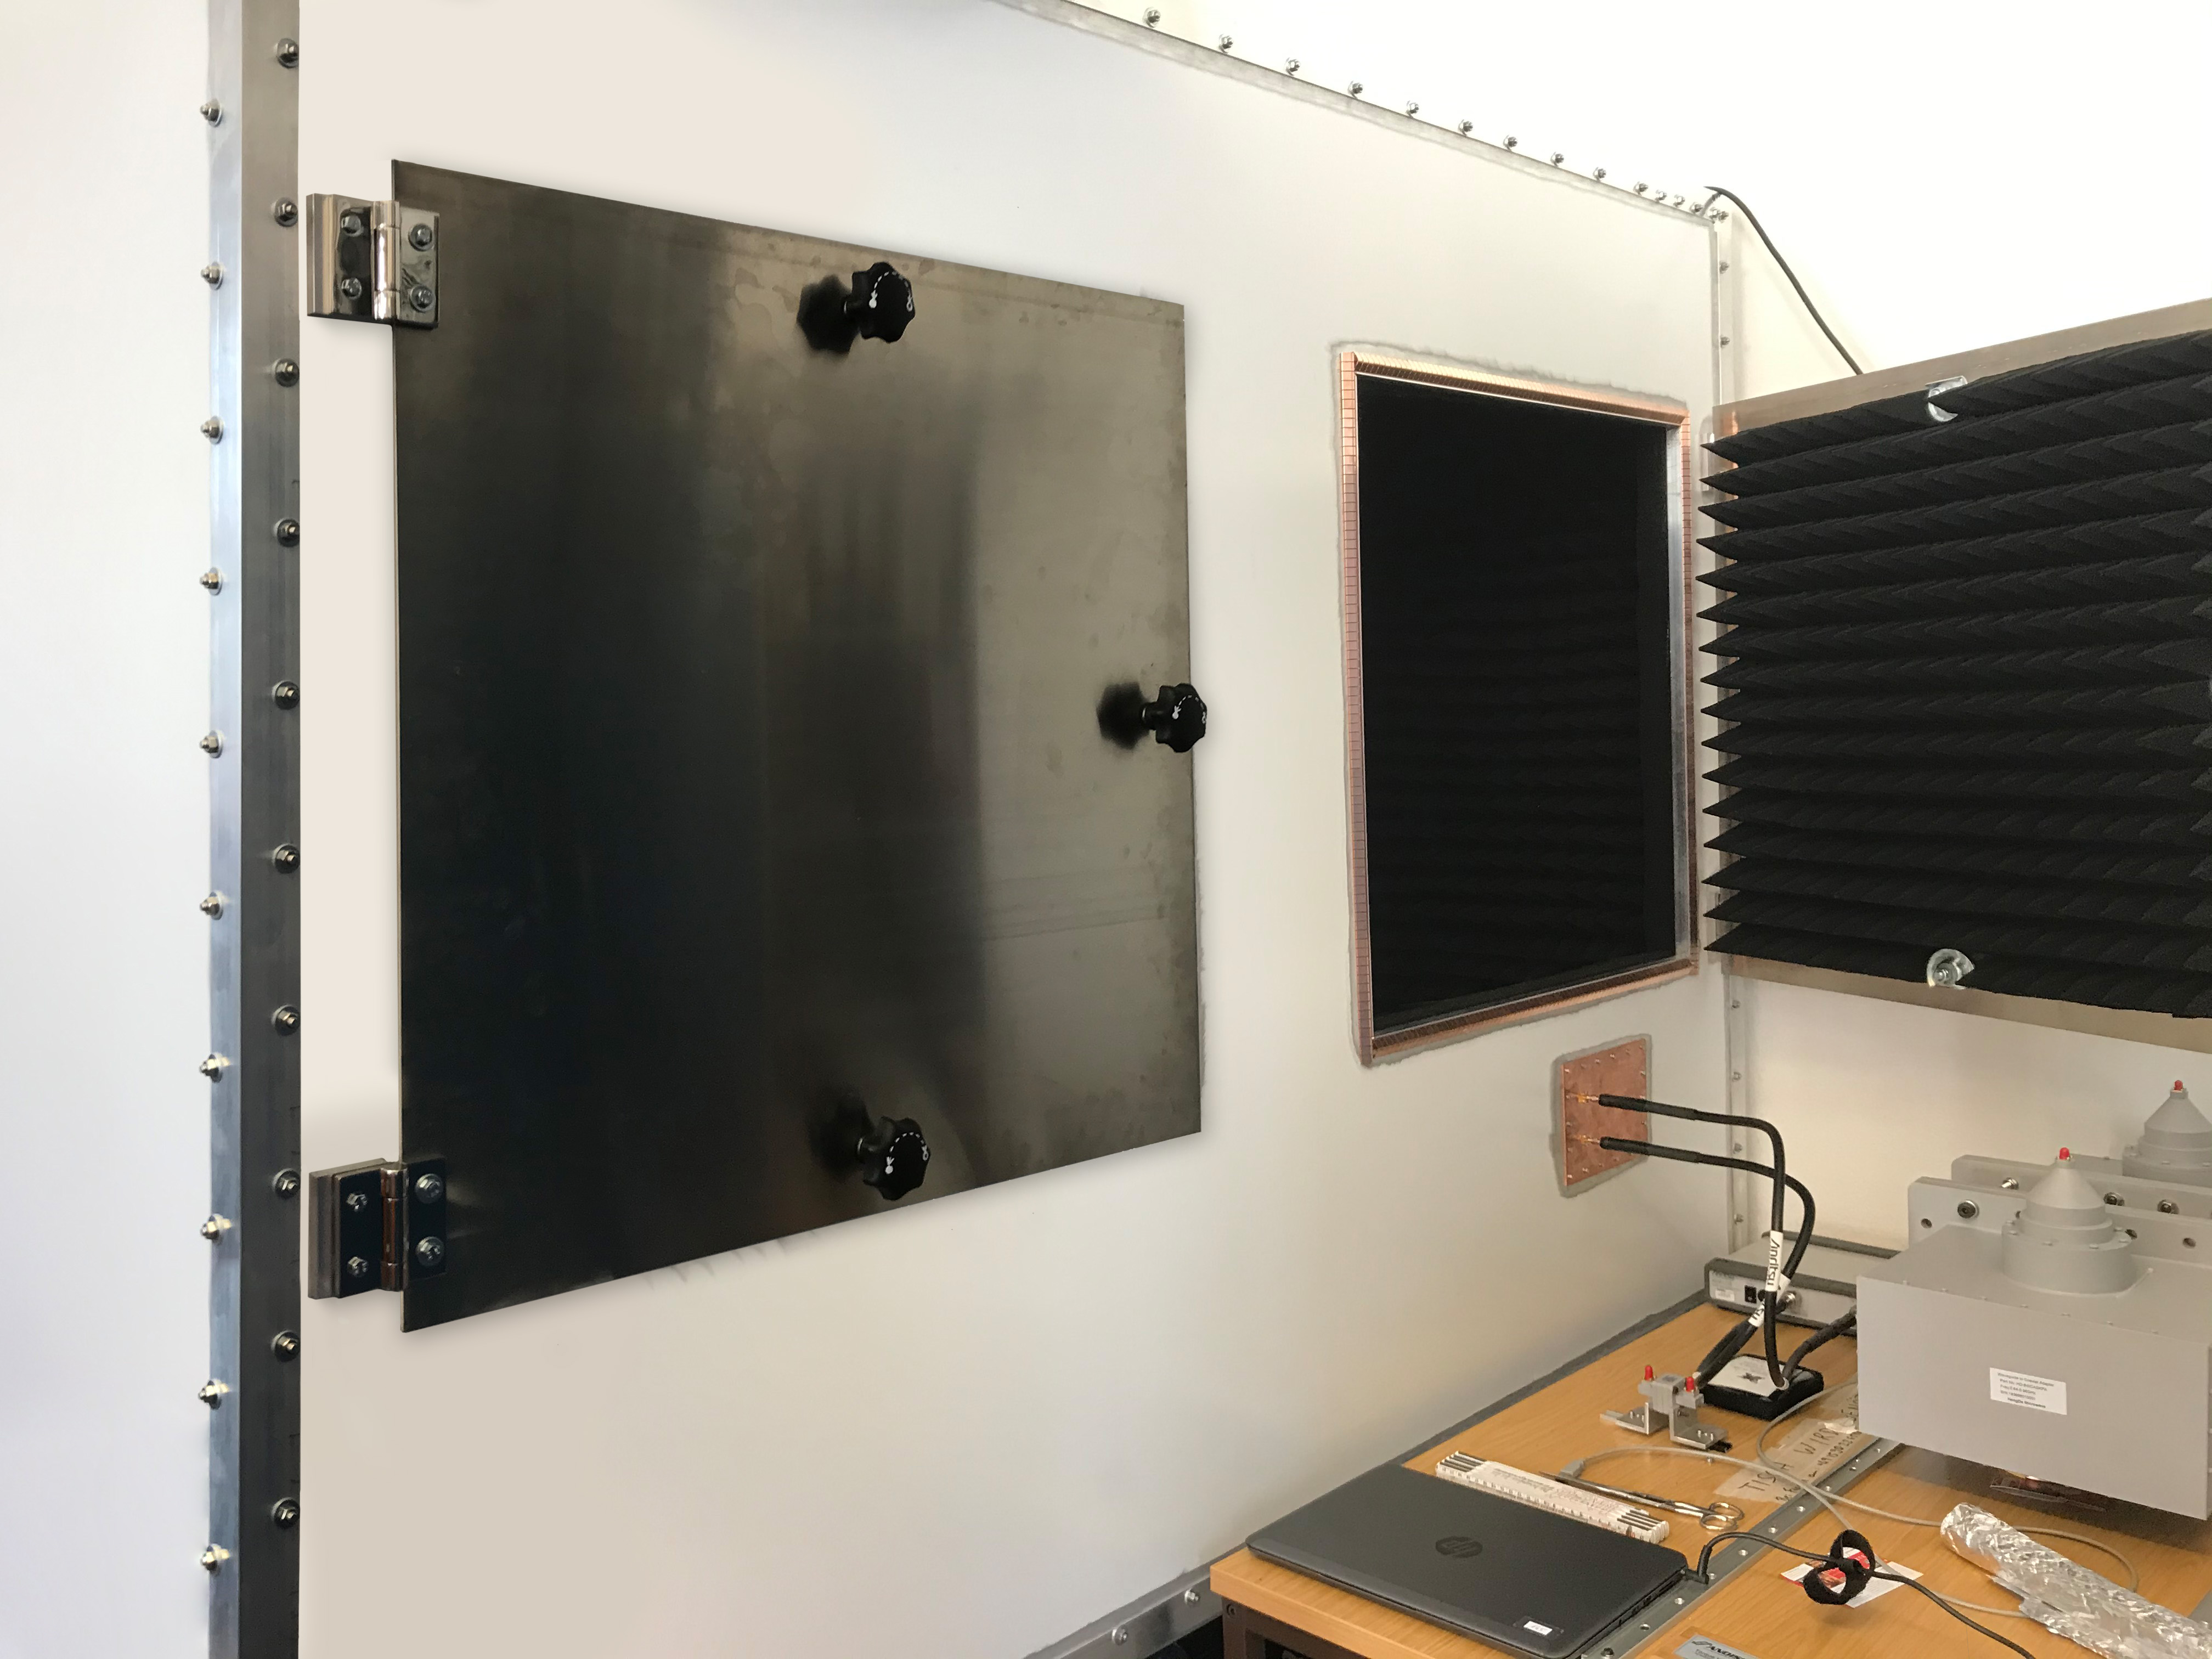
\includegraphics[height=.22\textheight, draft = false]{Abbildungen/Kapitel3/IMG_5467_bearbeitet.jpg}
    \hspace*{1cm}
    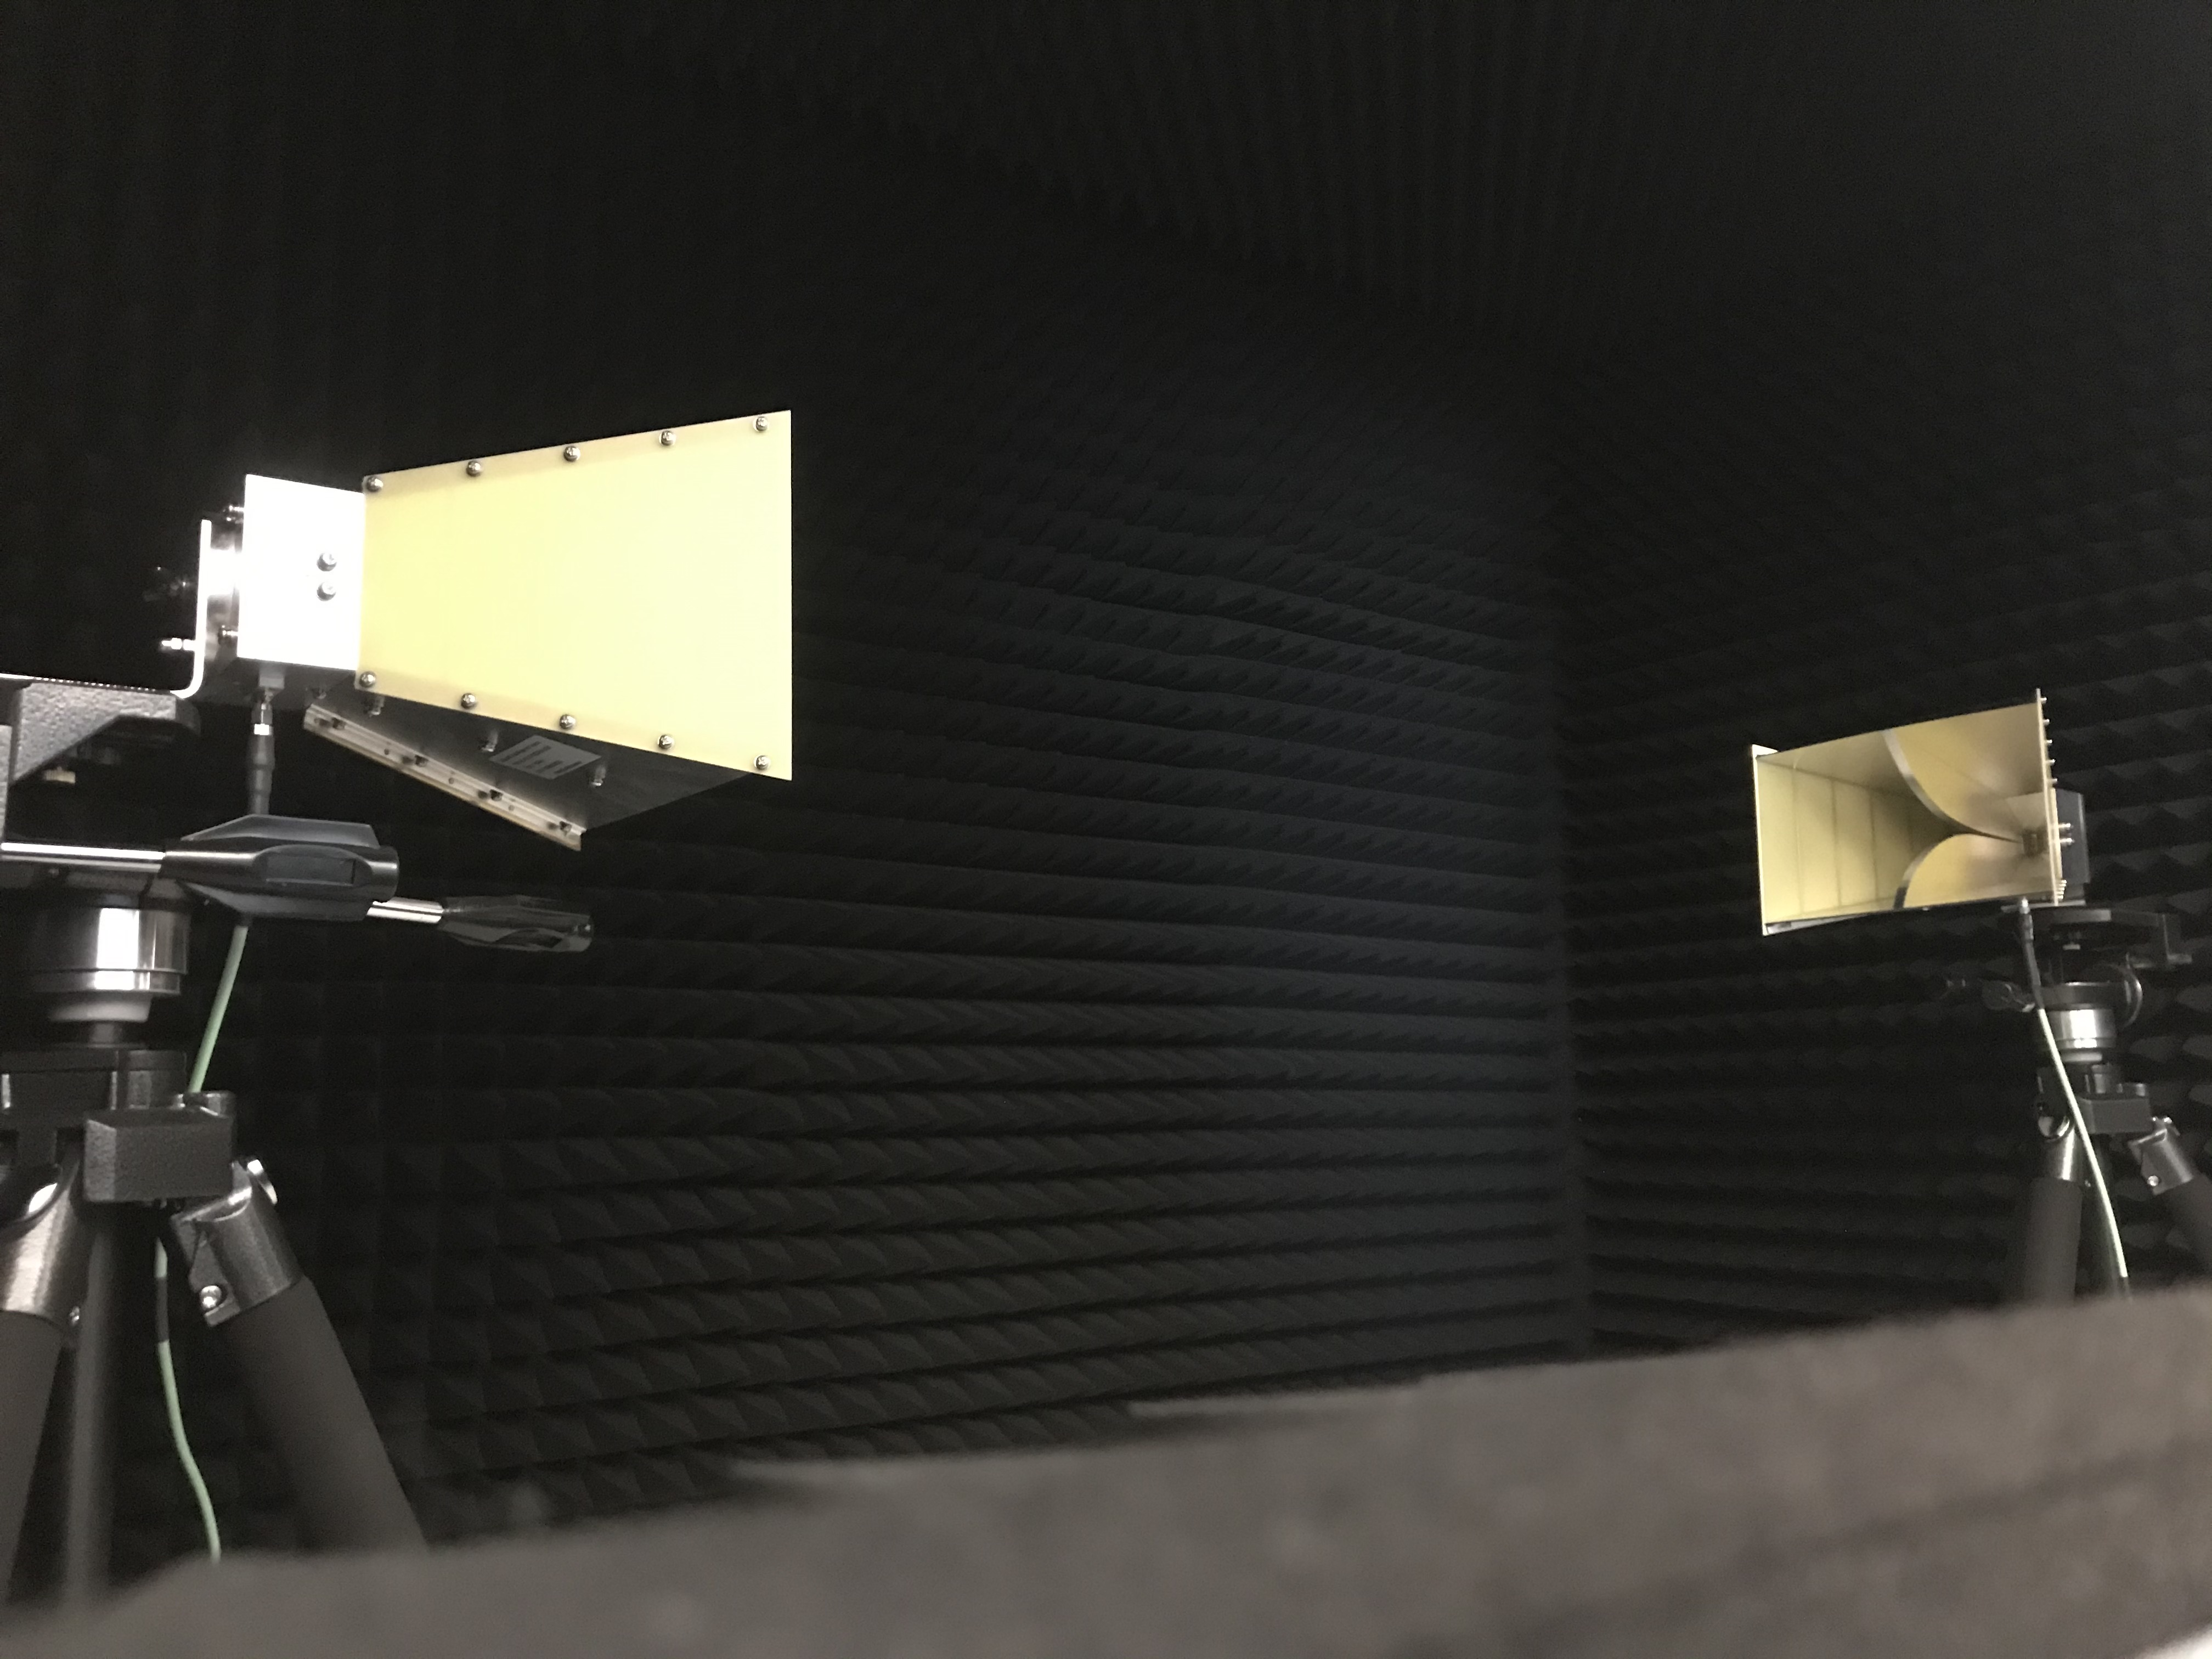
\includegraphics[height=.22\textheight, draft = false]{Abbildungen/Kapitel3/IMG_5472.jpg}
    \caption[Fernfeldversuchsstand von außen und Messstrecke]{Fernfeldversuchsstand von außen und Messstrecke mit Antennen}
    \label{fig:3_Gesamtversuchsstand}
\end{figure}



